
%(BEGIN_QUESTION)
% Copyright 2009, Tony R. Kuphaldt, released under the Creative Commons Attribution License (v 1.0)
% This means you may do almost anything with this work of mine, so long as you give me proper credit

Calculate the necessary piston diameter for this air-over-oil car lift to enable it to lift a 6,000 pound vehicle with a maximum applied air pressure of 100 PSI:

$$\includegraphics[width=15.5cm]{i03779x01.eps}$$

\vskip 20pt \vbox{\hrule \hbox{\strut \vrule{} {\bf Suggestions for Socratic discussion} \vrule} \hrule}

\begin{itemize}
\item{} Does the size of the oil reservoir matter in this calculation?  Why or why not?
\end{itemize}

\underbar{file i03779}
%(END_QUESTION)





%(BEGIN_ANSWER)

$$P = {F \over A}$$

$$A = {F \over P}$$

$$A = {6000 \hbox{ lb} \over 100 \hbox{ PSI}}$$

$$A = 60 \hbox{ in}^2$$

\vskip 10pt

$$A = \pi r^2$$

$$r = \sqrt{A \over \pi}$$

$$r = \sqrt{60 \hbox{ in}^2 \over \pi}$$

$$r = 4.37 \hbox{ inches}$$

So, the minimum piston diameter must be 8.74 inches.

%(END_ANSWER)





%(BEGIN_NOTES)


%INDEX% Physics, fluids: pressure, force, and area
%INDEX% Process: automobile hydraulic lift

%(END_NOTES)


